\documentclass[]{article}
\usepackage{fullpage}
\usepackage{graphicx}
\usepackage{xfrac}
%opening
\title{Electrical Conductivity Measurement of Various Cocktails \& Precursors}
\author{Carlos Gross Jones}

\begin{document}

\maketitle

\begin{abstract}
The electrical conductivities of numerous cocktails and precursors are measured, with a focus on predictability and reproducibility. Cocktails are evaluated and optimized for use in a magnetohydrodynamic cocktail stirrer. 
\end{abstract}

\section{Motivation}
\par In the initial FEA models for a contactless magnetohydrodynamic cocktail stirrer, one of the greatest uncertainties was the conductivity of the cocktail. Since the entire principle is based on the induction of currents in a liquid, the electrical resistance of the liquid is of great importance. Unfortunately, the author was unable to find previous experimental electrical data on alcoholic beverages and mixtures thereof. There is of course a body of electrochemical work on the ionic properties of pure ethanol (as well as other alcohols), but that is largely irrelevant. While pure ethanol is a very poor conductor, much like water, the important factor is the inclusion of other substances (flavor, or ``contaminants'' from a chemistry point of view).
\par Therefore, in order to analyze the practicality (or lack thereof) of the contactless cocktail stirrer, it is necessary to empirically determine the conductivity of the working fluid. In fact, to give the endeavor the greatest chances of success, the purpose of this segment is not only to measure the conductivity of a representative sample, but to \textit{optimize} for conductivity while still maintaining reasonable palatability.
\section{Theory}
\subsection{Sample Geometry}
\par In an infinite, homogeneous volume of a material with nonzero electrical conductivity, the electric field caused by two point voltages is of course easily solved, and the resultant current field (as a function of the conductivity, voltage, and distance between the points) can then be trivially computed. However, due to the economic impracticality of providing cocktails of infinite volume, it is preferable to use constrained geometry. For ease of calculation, it is best to restrict current flow to one dimension (i.e, uniform electric field between and normal to two identical charged conductive plates), allowing the resistance to be found as:
\begin{equation}
R=\frac{\ell}{A}
\end{equation}
where $\ell$ is the distance between the plates and $A$ is the plate area.

\subsection{AC Measurement}
\par Unfortunately, merely placing two metal plates in contact with the liquid under test and passing a DC current through it would not necessarily produce accurate results. First of all, electrolysis would take place, altering the chemical makeup of the sample; and second, most common electrode materials (such as copper) would undergo electrochemically-driven erosion, quickly contaminating the sample. Therefore, the electrodes must be coupled to the sample capacitively, and AC current used to characterize the conductivity. 
\par The sample can be seen as an ideal resistor, with series capacitors (representing the plate couplings) at either end. To complete the circuit, a second resistor is added in series, to be the other half of a resistor divider (Fig. \ref{fig:equivalent_circuit}).
\begin{figure}[h!]
	\centering
	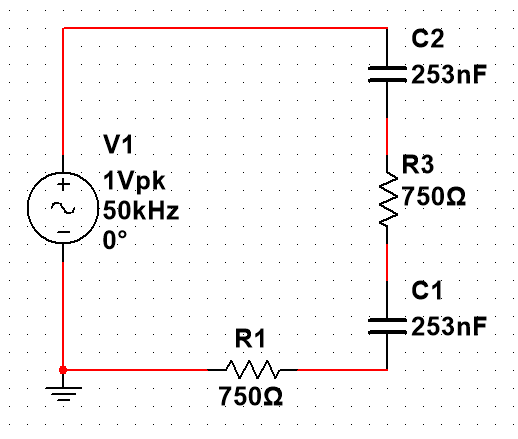
\includegraphics[width=0.3\textwidth]{Conductivity_Equivalent_Circuit}
	\caption{Equivalent Circuit}
	\label{fig:equivalent_circuit}
\end{figure}
When a known sinusoidal voltage is applied across the circuit, by measuring the voltage drop across the second (known) resistor, the impedance of the sample segment (resistive sample plus capacitive couplings) can be determined. From the properties of the materials making up the capacitor dielectrics and the area of the channel, the effective capacitance can be calculated, and thus their contribution to the impedance:
\begin{equation}
Z_c=\frac{-i}{2\pi f C}
\end{equation}
Subtracting the capacitive impedance, and approximating the sample fluid as purely resistive, its conductivity can then be calculated.
 \par To provide optimal sensitivity, the impedance of the capacitors should be as small as possible to reduce their contribution to the impedance of the sample segment. Modeling them as parallel-plate capacitors:
 \begin{equation}
 C=\epsilon\frac{A}{d}
 \end{equation}
 where $A$ is the plate area, $d$ the separation, and $\epsilon$ the permittivity of the dielectric, or equivalently:
 \begin{equation}
 C=\epsilon_R\epsilon_0\frac{A}{d}
 \end{equation}
with absolute permittivity replaced by the product of relative permittivity and the permittivity of free space.
The area of the capacitors is determined by the channel area, and the thickness and relative permittivity of the dielectric is limited by material choice. The remaining parameter, frequency, should be as high as possible without introducing significant parasitic RF effects. 50 kHz was chosen as the driving frequency.
\par To separate the sample from the electrodes, consumer Saran\textregistered film was chosen for its small thickness (nominally 0.0005'' thick). Chemically polyethylene, it has an $\epsilon_R$ of 2.25. Considering the plate dimensions to be nominally \sfrac{1}{2}'' by \sfrac{1}{2}'', the calculated capacitance is 253 nF, giving an impedance at 50 kHz of $-12.58 i\;\Omega$.
\par Preferably, the value of R1 should be close to R3 (the resistance of the sample); the greatest change in measured voltage across R1 per change in R3 (i.e., the measurement sensitivity) is provided when R1=R3. As a baseline, seawater ($\rho=0.2\:\Omega\cdot m$) was used to calculate a sample resistance of 756 $\Omega$. Therefore, a 750 $\Omega$ resistor was chosen for R1.
\section{Experimental Apparatus}
\par For the purposes of these experiments, a rectangular horizontal channel was chosen, with interior dimensions \sfrac{1}{2}'' wide by \sfrac{1}{2}'' tall, and 24'' long. Since the material forming the channel needs to be both waterproof and nonconductive,  ultra-high molecular weight polyethylene (UHMW) was chosen, in the form of a section of ``U'' stock (McMaster-Carr P.N. 9928K53). UHMW is electrically insulating, extremely nonporous and resistant to liquid absorption, and, as an added benefit, food-safe. The channel chosen has \sfrac{1}{2}'' inside dimensions and \sfrac{1}{4}'' thick walls. The channel is placed horizontally, for ease of use, with the conducting plates mounted at the ends. This leads to a channel 24'' long and \sfrac{1}{2}'' wide. Since it is impractical for the channel to be filled \textit{exactly} to the top with liquid, in practice the effective height will be slightly less than \sfrac{1}{2}'', with the actual liquid level being measured for each trial.
\section{Evaluation of Precursors}
\section{Development of Standard Cocktails}
\section{Results}
\subsection{Error Analysis}
\label{sec:error}

\end{document}
